% $Id: introduction.tex 1784 2012-04-27 23:29:31Z nicolas.cardozo $
% !TEX root = main.tex

\chapter{Identification and fixing of bugs}
\label{cha:features}

We now introduce the back-in time debugger using three examples of a Management Information System (MIS) that administers grades at a university in a similar fashion as it was done to explain DeloreanJS use cases, more on the actual complete code to solve the presented problems can be found at \url{https://github.com/af-orozcog/MVI-kotlin-examples}. The following figure shows the Intellij plugin in action

\begin{figure}[h]
\centering
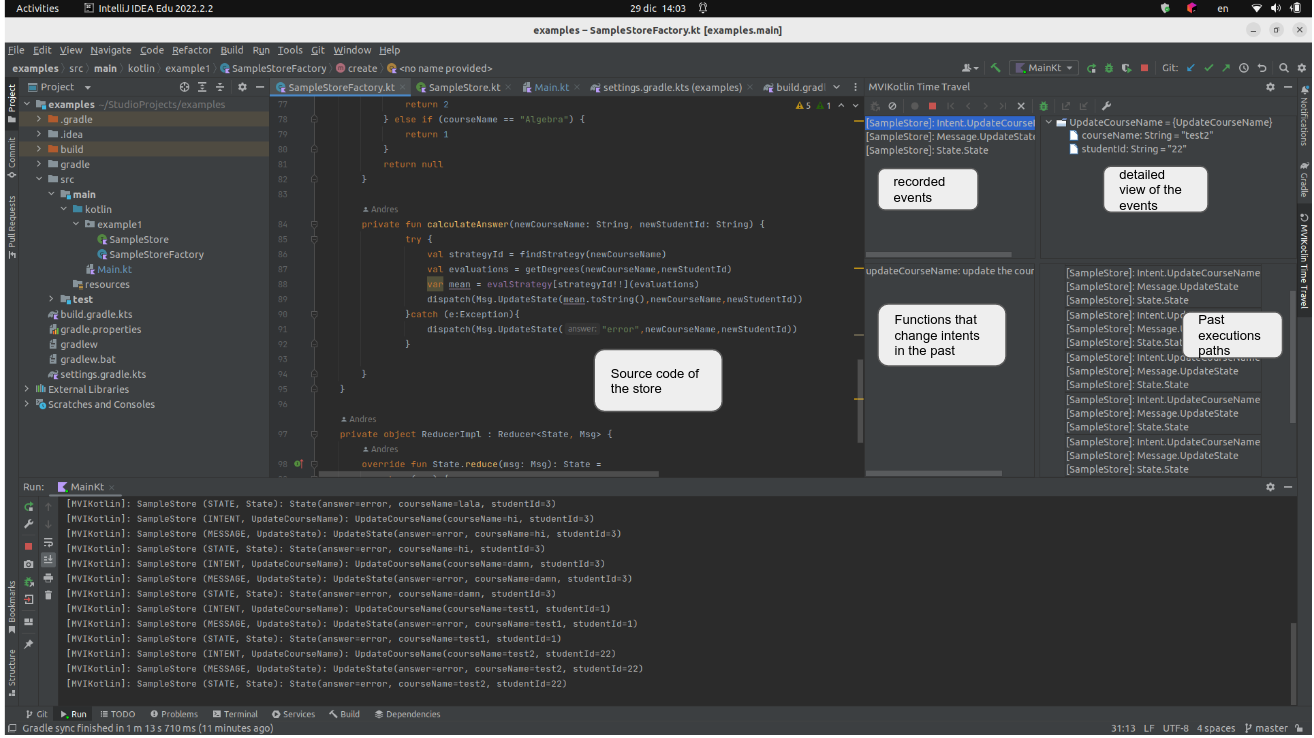
\includegraphics[height=7cm,width=13cm]{figures/Intellij}
\caption{A screenshot of the Intellij plugin}
\label{fig: A screenshot of the Intellij plugin}
\end{figure}

The plugin which is the main way to debug errors is composed of four panels, from left to right and top to bottom, the first panel shows the current events that are happening during the execution of the program. The second panel shows a detailed view of the events the user may wants to examine. The third panel shows the possible funtions that may be triggered to change the state of the program in a certain point on. The fourth panel shows all the previous executions paths of the program from most recent to oldest in a top to bottom fashion.

Given that most of the examples written for DeloreanJS did not have to comply with a reactive way of coding, the presented code will be an adaptation for the same problems written using reactive programming, which is based on events.

\section{Quick introduction to Stores}

In simple terms, \textbf{stores} are the objects that would enable use to go back in time. This is because they record for every moment in the program execution the state of a series of variables the developer has instructed to follow. They also provide the public functions that can be called by the coder to change the state of variables in the past.

\textbf{Stores} are the objects that will be used through the examples to record variables, they are defined by the coder and follow the MVI architectural pattern of programming. Nonetheless, most of the examples are illustrations of the use cases and do not represent a complete implementation and usage of the \textbf{stores}. More details on this can be found in the next chapter and in the github repository.

\section{Fix a bug}

A common task that is usually done by system that administers grades for a university is to calculate the final grade of the course. Notice that in order to calculate the final grade different rules may apply for different courses, so it is important to know which course the grades will be calculated for. In the following example, image that the course was incorrectly typed and an error would always trigger, because the course name was misspelled from "Algebra" to "Alggebra", then if the programmer could simply change the name of the course to the correct one, the bug would be fixed.

To be able to debug this type of event, a \textbf{store} will be created that accepts the courseName and courseId and according to that calculates the answer, which in this case is the final grade. The following is the Store interface:

\lstset{
  columns=fullflexible,
  frame=single,
  breaklines=true,
  postbreak=\mbox{\textcolor{red}{$\hookrightarrow$}\space},
}

\begin{lstlisting}[language=java]
internal interface SampleStore: Store<Intent,State, Nothing> {
    sealed class Intent : JvmSerializable {
        data class UpdateCourseName(val courseName: String, val studentId: String) : Intent()
    }

    data class State(
        val answer: String = "",
        val courseName: String = "",
        val studentId: String = ""
    ) : JvmSerializable // Serializable only for exporting events in Time Travel, no need otherwise.
}
\end{lstlisting}

Here we can see the store will receive an intent specifying the courseName and studentId to trigger the calculation of the grade. This calculation part is shown in the following piece of code where we define the executor, which is the component that reacts to intents.

\begin{lstlisting}[language=java]
override fun executeIntent(intent: Intent, getState: () -> State) {
   when (intent) {
       is Intent.UpdateCourseName -> calculateAnswer(intent.courseName, intent.studentId)
   }.let {}
}

private fun calculateAnswer(newCourseName: String, newStudentId: String) {
   try {
       val strategyId = findStrategy(newCourseName)
       val evaluations = getDegrees(newCourseName,newStudentId)
       var mean = evalStrategy[strategyId!!](evaluations)
       dispatch(Msg.UpdateState(mean.toString(),newCourseName,newStudentId))
   }catch (e:Exception){
       dispatch(Msg.UpdateState("error",newCourseName,newStudentId))
   }
}

\end{lstlisting}

In the previous piece of the code given an intent to update the courseName and studentId, a function calculateAnswer is called to update the answer variable to the corresponding value either the grade of the student, or record an error in the answer.

\section{Experiment with Hypothetical Scenarios}



\endinput

